%%%%%%%%%%%%%%%%%%%%%%%%%%%%%%%%%%%%%%%%%%%%%%%%%%%%%%%%%%%%%%%%%%
%%%%%%%%%%%%%%%%%%%%%%%%%%%%%%%%%%%%%%%%%%%%%%%%%%%%%%%%%%%%%%%%%%
%Packages
\documentclass[10pt, a4paper, twocolumn]{article}
\usepackage[top=3cm, bottom=4cm, left=2cm, right=2cm]{geometry}
\usepackage{amsmath,amsthm,amsfonts,amssymb,amscd, fancyhdr, color, comment, graphicx, environ}
\usepackage{float}
\usepackage{mathrsfs}
\usepackage[math-style=ISO]{unicode-math}
\setmathfont{TeX Gyre Termes Math}
\usepackage{lastpage}
\usepackage[dvipsnames]{xcolor}
\usepackage[framemethod=TikZ]{mdframed}
\usepackage{enumerate}
\usepackage[shortlabels]{enumitem}
\usepackage{fancyhdr}
\usepackage{indentfirst}
\usepackage{listings}
\usepackage{sectsty}
\usepackage{thmtools}
\usepackage{shadethm}
\usepackage{hyperref}
\usepackage{setspace}
\usepackage[linguistics]{forest}
\hypersetup{
    colorlinks=true,
    linkcolor=blue,
    filecolor=magenta,      
    urlcolor=blue,
}
%%%%%%%%%%%%%%%%%%%%%%%%%%%%%%%%%%%%%%%%%%%%%%%%%%%%%%%%%%%%%%%%%%
%%%%%%%%%%%%%%%%%%%%%%%%%%%%%%%%%%%%%%%%%%%%%%%%%%%%%%%%%%%%%%%%%%
%Environment setup
\mdfsetup{skipabove=\topskip,skipbelow=\topskip}
\newrobustcmd\ExampleText{%
An \textit{inhomogeneous linear} differential equation has the form
\begin{align}
L[v ] = f,
\end{align}
where $L$ is a linear differential operator, $v$ is the dependent
variable, and $f$ is a given non−zero function of the independent
variables alone.
}
\mdfdefinestyle{theoremstyle}{%
linecolor=black,linewidth=1pt,%
frametitlerule=true,%
frametitlebackgroundcolor=gray!20,
innertopmargin=\topskip,
}
\mdtheorem[style=theoremstyle]{Problem}{Problem}
\newenvironment{Solution}{\textbf{Solution.}}

\definecolor{codegreen}{rgb}{0,0.6,0}
\definecolor{codegray}{rgb}{0.5,0.5,0.5}
\definecolor{codepurple}{rgb}{0.58,0,0.82}
\definecolor{backcolour}{rgb}{0.95,0.95,0.92}

\lstdefinestyle{mystyle}{
    backgroundcolor=\color{backcolour},   
    commentstyle=\color{codegreen},
    keywordstyle=\color{magenta},
    numberstyle=\tiny\color{codegray},
    stringstyle=\color{codepurple},
    basicstyle=\ttfamily\footnotesize,
    breakatwhitespace=false,         
    breaklines=true,                 
    captionpos=b,                    
    keepspaces=true,                 
    numbers=left,                    
    numbersep=5pt,                  
    showspaces=false,                
    showstringspaces=false,
    showtabs=false,                  
    tabsize=2
}

\lstset{style=mystyle}
%%%%%%%%%%%%%%%%%%%%%%%%%%%%%%%%%%%%%%%%%%%%%%%%%%%%%%%%%%%%%%%%%%
%%%%%%%%%%%%%%%%%%%%%%%%%%%%%%%%%%%%%%%%%%%%%%%%%%%%%%%%%%%%%%%%%%
%Fill in the appropriate information below
\newcommand{\norm}[1]{\left\lVert#1\right\rVert}     
\newcommand\course{Materials, Sensors, Actuators & Fabrication in Robotics}  
\newcommand\hwnumber{ME5410}
\newcommand\teamnumber{Team 11}
\newcommand\Information{Name (ID): Bai Chengxi(), Cao Chenyu(), Hao Yuqi(), Li Zhangjin(), Miao Chenhui(), Zhou Yinhong()}                        % <-- personal information
%%%%%%%%%%%%%%%%%%%%%%%%%%%%%%%%%%%%%%%%%%%%%%%%%%%%%%%%%%%%%%%%%%
%%%%%%%%%%%%%%%%%%%%%%%%%%%%%%%%%%%%%%%%%%%%%%%%%%%%%%%%%%%%%%%%%%
%Page setup
\pagestyle{fancy}
\headheight 35pt
\lhead{\today}
% \rhead{
\includegraphics[width=2.5cm]{logo-nus.png}}
\lfoot{}
\pagenumbering{arabic}
\cfoot{\small\thepage}
\rfoot{}
\headsep 1.2em
\renewcommand{\baselinestretch}{1.25}
%%%%%%%%%%%%%%%%%%%%%%%%%%%%%%%%%%%%%%%%%%%%%%%%%%%%%%%%%%%%%%%%%%
%%%%%%%%%%%%%%%%%%%%%%%%%%%%%%%%%%%%%%%%%%%%%%%%%%%%%%%%%%%%%%%%%%
%Add new commands here
\renewcommand{\labelenumi}{\alph{enumi})}
\newcommand{\Z}{\mathbb Z}
\newcommand{\R}{\mathbb R}
\newcommand{\Q}{\mathbb Q}
\newcommand{\NN}{\mathbb N}
\newcommand{\PP}{\mathbb P}
\DeclareMathOperator{\Mod}{Mod} 
\renewcommand\lstlistingname{Algorithm}
\renewcommand\lstlistlistingname{Algorithms}
\def\lstlistingautorefname{Alg.}
\newtheorem*{theorem}{Theorem}
\newtheorem*{lemma}{Lemma}
\newtheorem{case}{Case}
\newcommand{\assign}{:=}
\newcommand{\infixiff}{\text{ iff }}
\newcommand{\nobracket}{}
\newcommand{\backassign}{=:}
\newcommand{\tmmathbf}[1]{\ensuremath{\boldsymbol{#1}}}
\newcommand{\tmop}[1]{\ensuremath{\operatorname{#1}}}
\newcommand{\tmtextbf}[1]{\text{{\bfseries{#1}}}}
\newcommand{\tmtextit}[1]{\text{{\itshape{#1}}}}

\newenvironment{itemizedot}{\begin{itemize} \renewcommand{\labelitemi}{$\bullet$}\renewcommand{\labelitemii}{$\bullet$}\renewcommand{\labelitemiii}{$\bullet$}\renewcommand{\labelitemiv}{$\bullet$}}{\end{itemize}}
\catcode`\<=\active \def<{
\fontencoding{T1}\selectfont\symbol{60}\fontencoding{\encodingdefault}}
\catcode`\>=\active \def>{
\fontencoding{T1}\selectfont\symbol{62}\fontencoding{\encodingdefault}}
\catcode`\<=\active \def<{
\fontencoding{T1}\selectfont\symbol{60}\fontencoding{\encodingdefault}}

%%%%%%%%%%%%%%%%%%%%%%%%%%%%%%%%%%%%%%%%%%%%%%%%%%%%%%%%%%%%%%%%%%
\usepackage{tabularx}
\usepackage{tikz}
\usetikzlibrary{shapes, arrows, positioning}
\usepackage{graphicx}
%%%%%%%%%%%%%%%%%%%%%%%%%%%%%%%%%%%%%%%%%%%%%%%%%%%%%%%%%%%%%%%%%%
%Begin now!



\begin{document}

\begin{titlepage}
    \begin{center}
        \vspace*{3cm}
            
        \Huge
        \textbf{Chess Playing Robot}
            
        \vspace{1cm}
        \huge
        \hwnumber
            
        \vspace{1.5cm}
        \Large

        \textbf{\teamnumber}
        
        \vspace{1.5cm}
        \Large
        
        \textbf{\Information}                      % <-- author
        
            
        \vfill
        
        % \course
            
        \vspace{1cm}
            
        
\includegraphics[width=0.4\textwidth]{logo-nus.png}
        \\
        
        \Large
        
        \today
            
    \end{center}
\end{titlepage}

%%%%%%%%%%%%%%%%%%%%%%%%%%%%%%%%%%%%%%%%%%%%%%%%%%%%%%%%%%%%%%%%%%
%Complete the assignment now
\begin{abstract}
During a chess match, a young player was unexpectedly injured when the chess-playing robot, as the opponent, grabbed and squeezed their finger. This incident drew widespread attention, highlighting the growing integration of robotics into human life and the urgent need for systematic optimization of robots to reduce potential harm to humans. 

This report explores strategies for optimizing chess-playing robots from multiple dimensions. Our research identifies two main risks: injuries from the robot's arm movement and accidental gripping of a human hand by the robot's end effector. To mitigate these risks, we propose optimizations in the robot's structural design and sensor detection. We reduced the robot's degrees of freedom, chose a high-precision gantry robot, and adjusted materials for a lightweight design. The end effector's structure was redesigned with a dual layer of soft and hard materials, reducing injury risk during accidental contact. Additionally, sensors were embedded for environmental monitoring to enhance safety. 

These measures aim to significantly improve the safety of chess-playing robots, ensuring smooth and secure human-robot interaction.
\end{abstract}

\section{Mini Review in Chess-Playing Robots}

\subsection{Actuators in Chess-Playing Robots}
For actuators, high-torque DC motors, precision step motors, and servo motors are crucial for accurate and controlled movements. They are used in designs such as the custom mid-cost 6-DoF (Degrees of Freedom) manipulator system called Gambit, which is capable of playing in non-idealized environments\cite{Gambit}. Another instance is the SCARA robot arm analyzed for its mechanical design and control algorithms to execute chess moves\cite{anh2016design}. The use of electromagnets to move pieces from underneath has also been documented, providing a different approach to piece manipulation\cite{chess_playing_robot_vub}.

\subsection{Sensory Systems in Chess-Playing Robots}
In terms of sensory systems, advanced cameras are integral for vision sensors, enabling the detection of the chessboard and piece positions. For instance, a computer vision algorithm has been developed that detects the board, squares, and piece positions, even in unconstrained environments, adjusting dynamically to changes in lighting and accounting for perspective distortion\cite{chen2019robust}. Additionally, the implementation of force sensors ensures the correct pickup and placement of pieces, as they provide feedback on the grip and force exerted\cite{omarsdottir2016axiomatic}.

Advanced systems may also incorporate artificial neural networks for enhanced efficiency in the recognition of chess states and possible moves, and collaborative robots have been used for playing chess, capable of tracking the state of the game\cite{kolosowski2020collaborative}.

\subsection{Features}
The mini review on the features of existing chess-playing robots has highlighted some common characteristics and functionalities:

\begin{enumerate}
    \item \textbf{Gantry Structure}:Chess-playing robots often employ a gantry structure due to its simplicity and accuracy in control. This structure is less complex than that of a mechanical arm, reducing the degrees of freedom and simplifying the control calculations and mathematical models.\cite{rao2023robot}
    
    \item \textbf{Linear X, Y, and Z-Axis Movement}: These robots typically have three degrees of freedom, corresponding to the X, Y, and Z axes, with each axis being an independent motion unit that performs linear movements. This characteristic is part of the gantry robot design and helps to lessen the computational load on the control system.\cite{du2013compliance}\cite{gupta2015autonomous}

    \item \textbf{Rigid Gripper}: The end effector or gripper of these robots is usually constructed from rigid materials such as steel or alloys, providing stability when handling chess pieces. However, the rigidity also poses a safety risk to human operators, as body parts like fingers can be injured by the mechanical pressure exerted by the grippers.
\end{enumerate}

The specifics of these features can vary between different chess-playing robots, but the overarching principles of gantry structure, linear movement, and robust grippers seem to be common in their design to ensure precise and efficient play against human opponents.

For further detailed information and technical specifications, it is recommended to review the cited sources and explore the references provided within them, such as technical papers and project repositories.

\subsection{Material}
In this course, the main robot materials used include the following: metal materials, polymer materials, ceramic materials, and composite materials.

Robots are crafted using metals like aluminum, steel, titanium, and copper for their robustness, forming key elements like skeletons and gears. Ceramics, such as aluminum oxide and silicon nitride, cater to high-temperature and chemically demanding parts like sensors. For lightweight, high-strength components, composites like carbon fiber are employed, merging multiple material benefits into robot structures.\cite{nelson_csc297_materials}

Polymer materials have lightweight, plasticity, and insulation properties, making them commonly used in robot casings, covers, and sensor packaging. They are used as materials for the shell and soft gripper of chess robots. The ABS plastic used in the shell is a common robot material that has advantages in weight, safety, durability, and other aspects. Soft pneumatic actuators (SPAs) are engineered to replicate human muscular structures, necessitating materials with high elasticity and resilience\cite{Rus2015}. Silicon rubber, polyurethane, fluor elastomers and thermoplastic elastomers are typical examples of elastomers in use.  Elastomers, which have garnered significant research interest\cite{Moseley2016}, are commonly employed due to their elastic properties. Silicon rubber is favored for its versatility and endurance, especially in applications demanding substantial stretch and adaptability\cite{Xavier2022}.

\begin{figure}
    \centering
    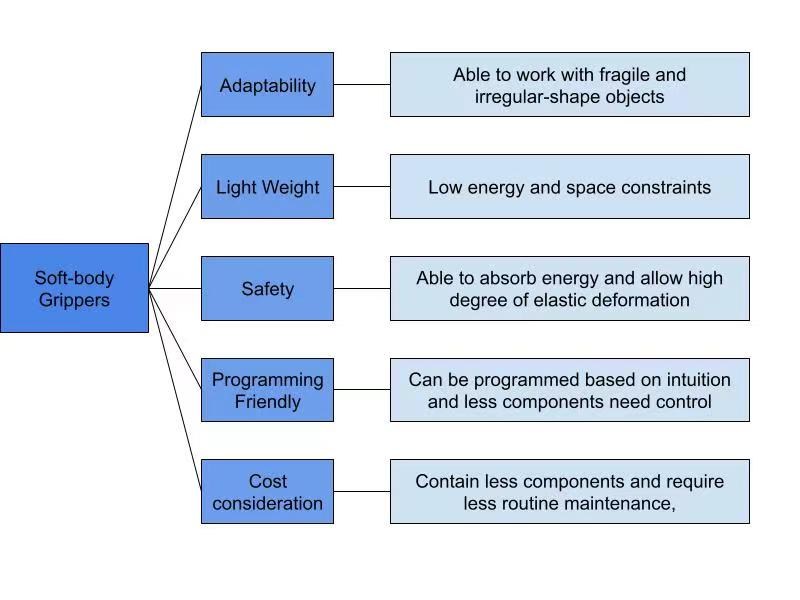
\includegraphics[width=1\linewidth]{advantages of soft-body grippers.jpg}
    \caption{advantages of soft-body grippers}
    \label{fig:advantages of soft-body grippers}
\end{figure}

\subsection{Fabrication}
The manufacturing process of chess-playing robots, particularly in the context of forming and assembly, has been augmented significantly with advancements in robotics and AI. For instance, Machina Labs in California utilizes AI and robotics to transform the sheet-forming industry. Their systems, featuring two 7-axis arms, enable the forming of metal sheets with remarkable precision and efficiency\cite{Khalid2023}. The comprehensive system autonomously manages loading, forming, scanning, cutting, finishing, and unloading, catering to the production of complex parts with high quality and repeatability, crucial for sectors like aerospace and automotive. These advancements result in shorter lead times, as the robots can operate continuously without the need for design-specific tooling or manual supervision\cite{harfoush2021application}.

In assembly, the role of robotics has become increasingly pivotal. Modern robots are flexible, autonomous, and capable of performing with minimal human intervention. They handle material transfer, loading, and unloading tasks, with complex operations like organizing parts on pallets. Processing tasks performed by robots include welding and painting, with precise operation leading to improvements in quality and production costs. In the assembly and inspection processes, robots can batch-produce various styles of a product and are programmed to adapt to different designs, optimizing efficiency and reducing the need for skilled human labor. For instance, in the Tesla Gigafactory, Autonomous Indoor Vehicles (AIVs) operate spontaneously, moving items between workstations, showcasing the potential of collaborative systems where robots and humans work in tandem\cite{RobotsNet2019}.

Incorporating these insights, the mini-review on the fabrication of chess robots could be enhanced by emphasizing the role of advanced robotics in both the forming and assembly stages, highlighting the benefits of precision, efficiency, and safety introduced by these technologies. This would not only give a comprehensive view of current practices but also shed light on the potential for future advancements in the field.

\section{Introduction to Principles}
\subsection{Transmission Principle}
The chess-playing robot mainly consists of three parts: the frame structure, the sliding rail moving mechanism, and the end effector. Other components include the motor and driving device. This robot, similar to existing three-coordinate gantry robots, features a "gate"-shaped frame as its supporting structure, providing ample stability and workspace, convenient for chessboard setup and player operation. The sliding rails mounted on the frame allow the end effector to move along three spatial axes (X, Y, Z axes).

The robot's moving mechanism is driven by a synchronous belt linear drive module, which consists of a synchronous belt, sliding rails and blocks, drive and driven wheels, an electric motor, brackets, and fasteners.

\begin{figure}
    \centering
    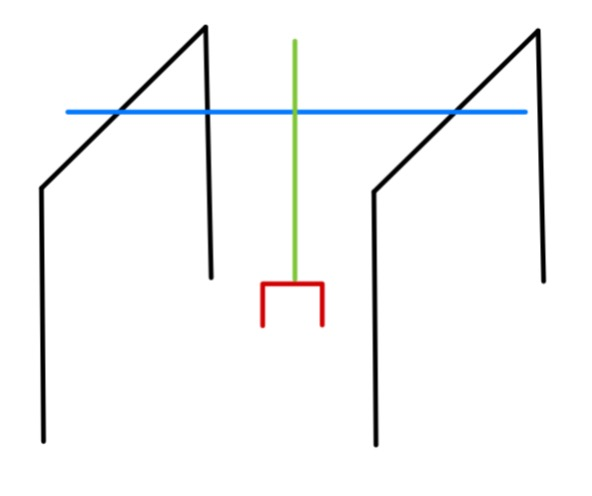
\includegraphics[width=0.5\linewidth]{schematic diagram.jpg}
    \caption{schematic diagram of "gate"-shaped frame}
    \label{fig:schematic diagram}
\end{figure}

\begin{figure}
    \centering
    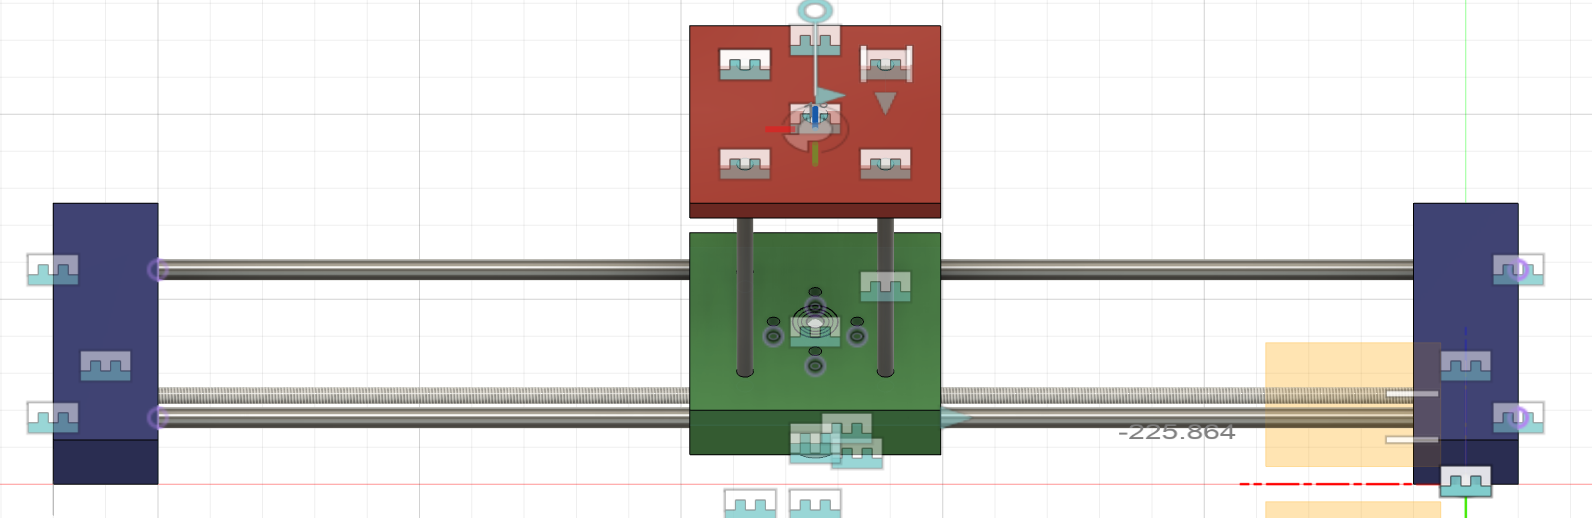
\includegraphics[width=0.8\linewidth]{screw drive in x-axis motion.png}
    \caption{screw drive in x-axis motion}
    \label{fig:screw drive in x-axis motion}
\end{figure}

\begin{figure}
    \centering
    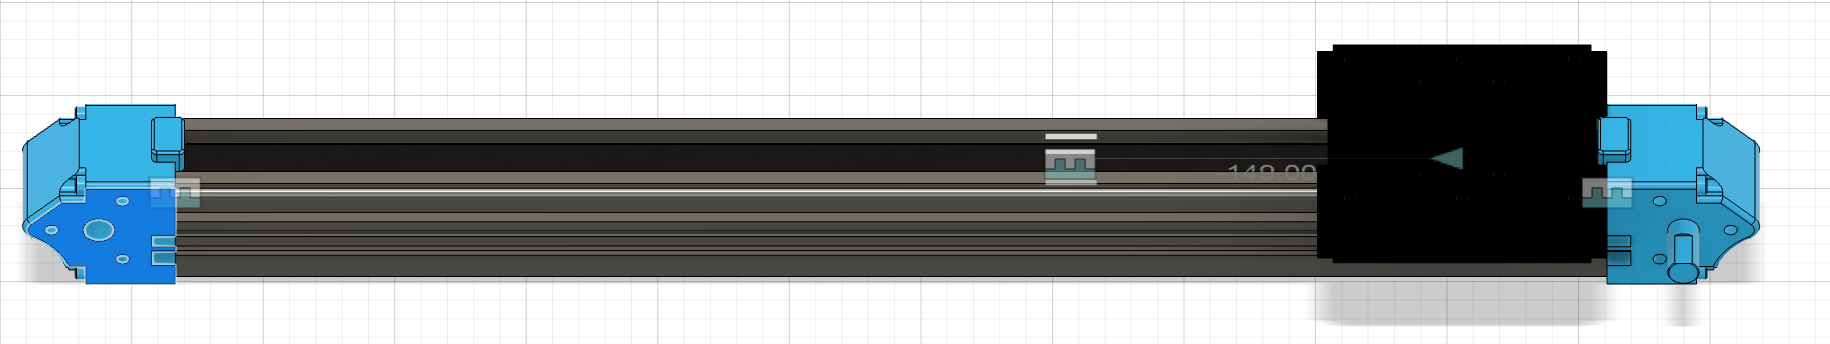
\includegraphics[width=0.8\linewidth]{belt drive in y-axis motion.png}
    \caption{belt drive in y-axis motion}
    \label{fig:belt drive in y-axis motion}
\end{figure}

This module exhibits the following characteristics:

\begin{itemize}
    \item \textbf{High Precision Positioning}: The synchronous belt drive enables high-precision positioning control, which is ideal for accurately positioning the end effector to the specific row or column of a chess piece on the board.
    \item \textbf{Low Noise and Smooth Operation}: Due to the smooth transmission of the synchronous belt, this drive module operates with low noise, meeting the environmental requirements for the activity of playing chess.
    \item \textbf{High Efficiency and Low Maintenance}: The transmission efficiency of the synchronous belt is high, and unlike chain drives, it does not require regular lubrication, thus reducing maintenance needs.
    \item \textbf{Customizability and Cost-Effectiveness}: This module can be manufactured in various lengths and widths to meet different application needs. Compared to other types of linear drive systems (such as ball screw drives), the synchronous belt linear drive module is usually more economical, allowing for mass custom production.
\end{itemize}

\begin{figure}
    \centering
    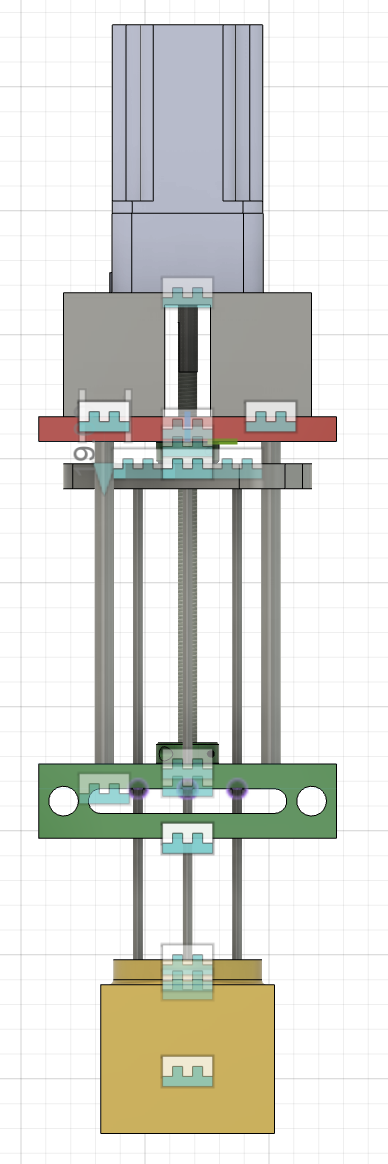
\includegraphics[width=0.25\linewidth, angle=90]{screw structure in z-axis motion.png}
    \caption{screw structure in z-axis motion}
    \label{fig:screw structure in z-axis motion}
\end{figure}

Due to the need for high positioning accuracy and repeatability in moving to the chess piece's position and grasping it, a screw structure with higher precision compared to the synchronous belt linear drive module is chosen as the up-and-down driving device for the end effector. This structure includes a central spiral screw and several pillars for supporting and guiding the moving parts. The drive motor (usually a stepper or servo motor) is located at the top of the lifting device and at the end of the sliding rail. It guides the movement of the end effector relative to the Y and Z axes of the chessboard by rotating the spiral screw, thus accurately reaching the position to grasp the chess pieces.

\begin{figure}
    \centering
    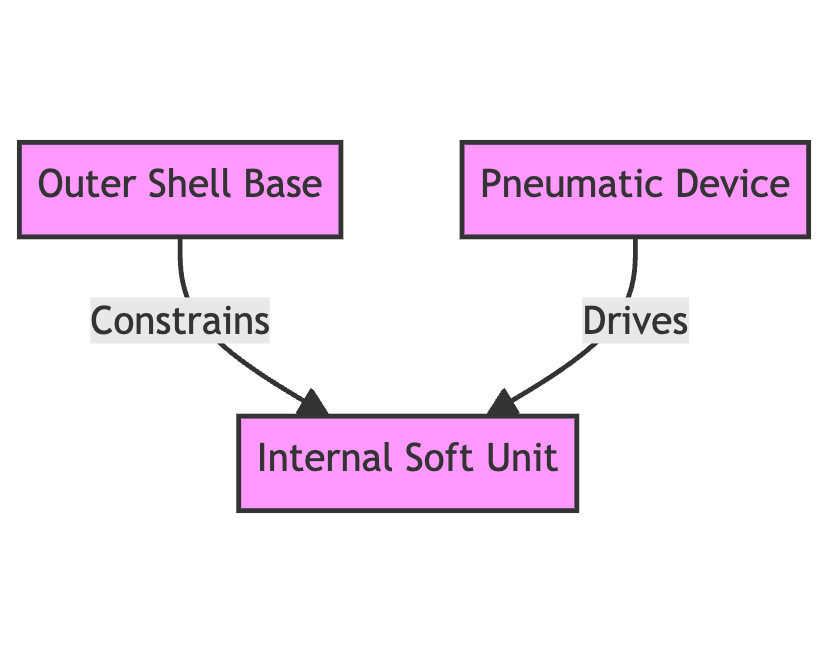
\includegraphics[width=0.6\linewidth]{grasping principle.png}
    \caption{schematic diagram of grasping principle}
    \label{fig:grasping principle}
\end{figure}

\subsection{Grasping Principle}
The grasping principle of a pneumatic soft robotic arm involves the transformation of air pressure into mechanical movement to achieve object manipulation. This process is typically realized through an end effector designed to mimic the adaptive grip of human fingers but using soft, flexible materials.

\begin{figure}[H]
\centering
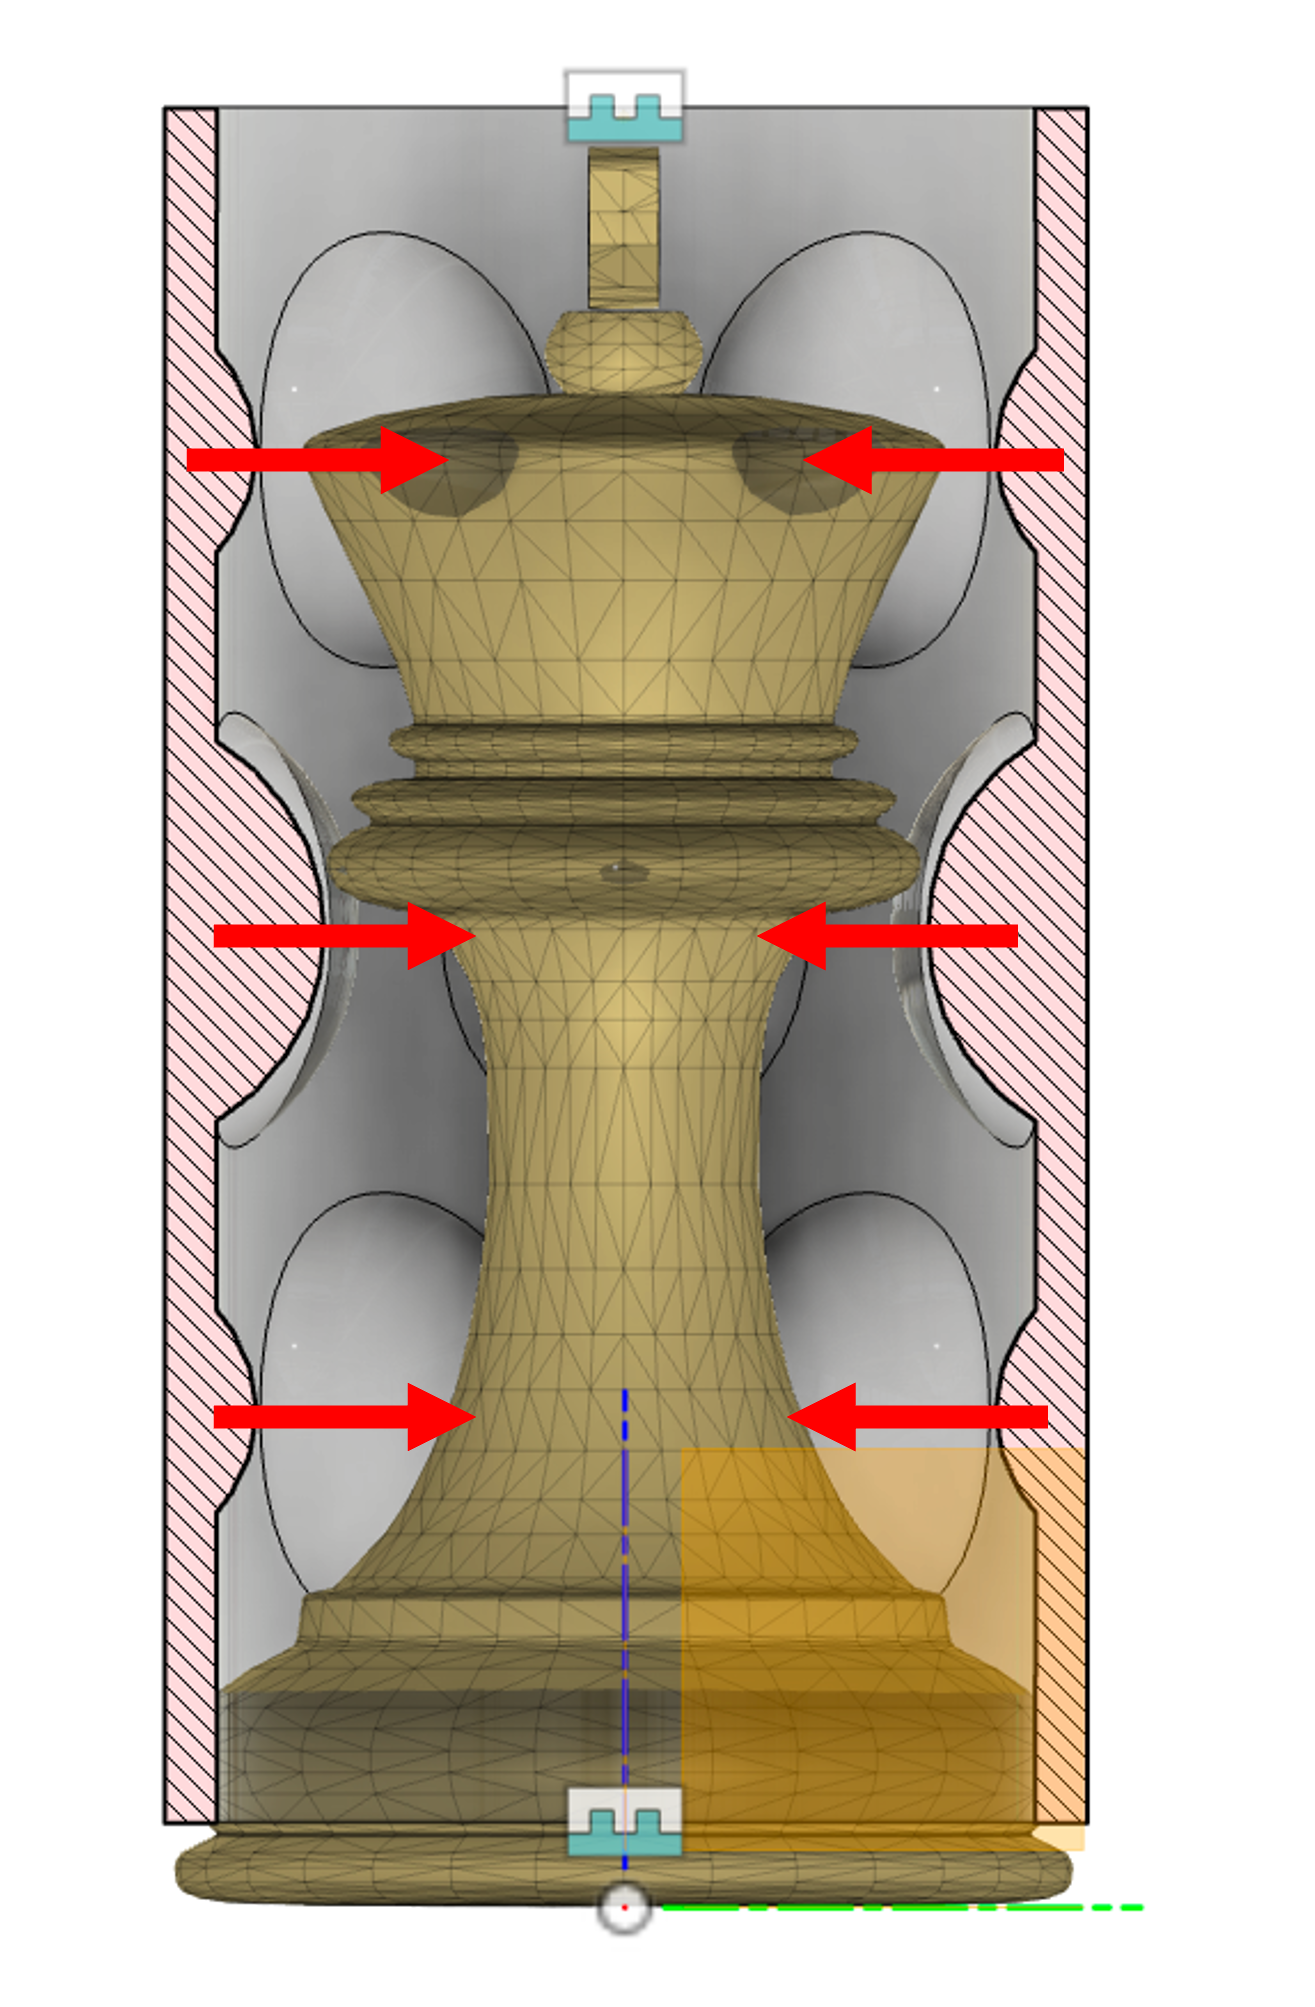
\includegraphics[width=0.3\linewidth]{grasping chess.png}
\caption{The principle of grasping a chess piece is demonstrated by the strategic inflation of the soft chambers within the arm, allowing for a gentle yet firm grip that conforms to the shape of the object.}
\label{fig:grasping_chess}
\end{figure}

In Figure \ref{fig:grasping_chess}, we see an example of a soft robotic end effector as it engages with a chess piece. The end effector's design allows for a controlled grasp, which is essential for handling objects of various sizes and fragility without causing damage. The inflation of the arm's chambers is carefully calibrated to exert just enough force to hold the piece securely without crushing it.

\begin{figure}[H]
\centering
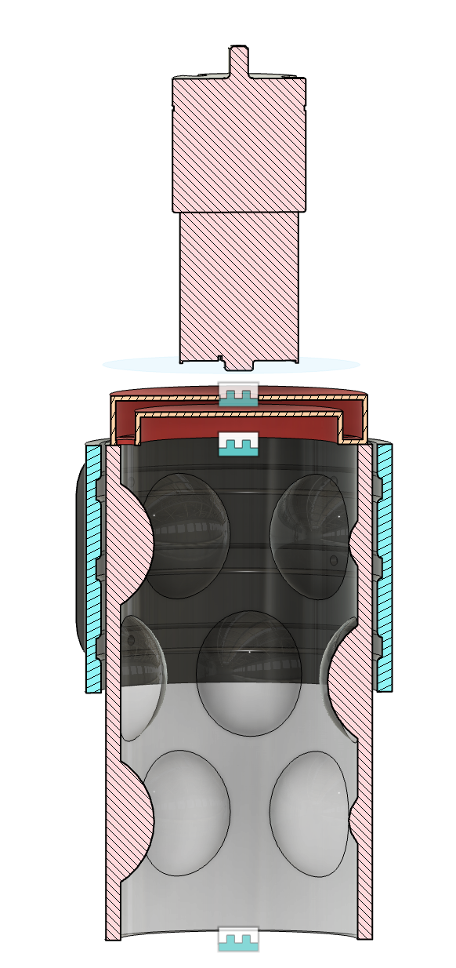
\includegraphics[width=0.3\linewidth]{end effector.png}
\caption{This figure illustrates the end effector structure, highlighting the flexible bladders or chambers that expand upon pneumatic actuation to engage with and encompass the object to be grasped.}
\label{fig:end_effector}
\end{figure}

Figure \ref{fig:end_effector} showcases the detailed structure of the end effector. The design often includes several chambers that can be independently inflated to adjust the shape and stiffness of the arm, allowing for a versatile gripping capability. This modularity in design makes it possible for the robotic arm to perform a wide range of tasks by changing the pattern of inflation to suit the specific object and task requirements.

\section{Control Principle}

This report delineates the principal components of the control system for a chess-playing robot, specifically focusing on its sensing and actuation mechanisms.

\subsection{Sensing System}

\begin{itemize}
    \item \textbf{Visual Recognition}: Employing cameras, the system captures the chessboard state, determining piece positions and possible moves. Image processing, potentially enhanced by multiple camera angles, discerns piece types and checks for human interaction to enhance safety.
    \item \textbf{Sensors}: A suite of sensors, including motion vectors and force detectors on the robot's effector, provides environmental feedback and interaction status, ensuring correct piece manipulation and human safety.
    \item \textbf{Computational Analysis}: The integration of software and machine learning algorithms processes visual data, improving recognition efficiency and adjusting to varying game setups.
\end{itemize}

\subsection{Actuator System}

\begin{itemize}
    \item \textbf{Precision Motors}: Utilizing servo motors with integrated encoders, the robot achieves precise control over its mechanical movements, vital for accurate positioning of its components.
    \item \textbf{Motor Control}: Advanced algorithms within the servo control system translate sensory inputs into meticulous motor operations, optimizing movement trajectories and exerted forces.
    \item \textbf{Pneumatic Actuation}: The Pneumatic Control Unit, powered by a high power-density SIMILK DC 6V air pump, manages the robot's soft actuators. Coupled with proportional valves and precise pressure sensors, it ensures the smooth operation of the actuation system.
\end{itemize}

\subsection{Implementation of Safety}
Firstly, we have focused on improving the structure of the end effector by using a soft actuator and covering the bottom of the actuator with a soft material to make it less likely to cause injury. Additionally, a capacitive distance sensor is installed at the position of the end effector to detect the proximity of human hands.

On the other hand, visual sensors and image recognition software are used to ensure that the entire robot stops moving once a human hand enters the chessboard area. The robot is also equipped with an emergency stop button, allowing for manual shutdown in urgent situations.

\section{Material Selection}
When selecting materials for manufacturing robots, considering the application scenarios and functional requirements, the commonly used materials include several categories: metals, plastics and synthetic materials, composite materials, flexible materials, and smart materials.

For this project's chess-playing robot, which primarily consists of three parts: the frame structure, the sliding rail moving mechanism, and the end effector, we decided to choose materials according to the different parts of the robot.

\subsection{Frame Structure and Sliding Rail Moving Mechanism}
We have chosen to use aluminum alloy for the frame structure and sliding rail moving mechanism, as aluminum alloy has the following advantages compared to other materials:

\begin{itemize}
    \item \textbf{Lightweight}: Aluminum alloy has a low density and is lightweight, which means the constructed frame structure and sliding rail moving mechanism will be relatively light. For the chess-playing robot, which may need to be moved frequently, this imposes certain limitations on the overall weight of the robot. Moreover, if the robot is too heavy, the impulse of the moving arm will be relatively large, which could cause injury if it comes into contact with a person during movement. Therefore, choosing lightweight aluminum alloy as the primary material for its structure is a good choice.
    \item \textbf{High Strength}: Despite its lightness, aluminum alloy has high strength and stiffness. The load of the chess-playing robot is relatively small, so using aluminum alloy meets the strength requirements of the robot well.
    \item \textbf{Good Machinability}: Aluminum alloy is easy to process and shape. It can be processed into various shapes through cutting, welding, casting, and other methods, making it convenient to manufacture the structure.
    \item \textbf{Economical}: Compared to other metal materials, the cost of aluminum alloy is relatively low, allowing for reduced manufacturing costs without sacrificing performance.
\end{itemize}

\subsection{End Effector}
The end effector of the chess-playing robot consists of two parts: the outer shell's base part and the internal soft pneumatic actuator. For these two parts, we have also chosen materials for manufacturing.

We have decided to use ABS to make the base part of the outer shell. ABS material has several advantages over other materials:
\begin{itemize}
    \item \textbf{Raw Material Cost}: The price of ABS plastic is generally lower than that of most metal materials, especially high-performance metals like aluminum alloys or stainless steel.
    \item \textbf{Manufacturing Speed}: Injection molding can rapidly produce a large number of parts, significantly increasing production efficiency and reducing unit costs.
    \item \textbf{Ease of Assembly}: ABS parts are usually easier to assemble because they can be designed with snaps, joints, etc., without the need for welding or complex machining.
\end{itemize}

For the internal soft pneumatic actuator, we choose to use Eco-flex, a highly elastic silicone material. As a primary material in the field of soft robotics, Eco-flex has the following advantages:
\begin{itemize}
    \item \textbf{High Flexibility}: It can be stretched many times its original size without tearing or deforming. This is beneficial for the application of the end effector of the chess-playing robot.
    \item \textbf{Biocompatibility}: Some grades of Eco-flex are biocompatible, meaning they can be safely used in applications that require direct contact with human skin.
    \item \textbf{Ease of Manufacture}: Eco-flex can be easily molded and cast into complex shapes, which is very convenient for production. 
\end{itemize}

\section{Manufacturing Methods}

As depicted in Fig. \ref{fig:final design}, we present the finalized design of the chess-playing robot. The manufacturing methodologies for the robot will be delineated separately for its frame structure and the end effector:

\begin{figure}
    \centering
    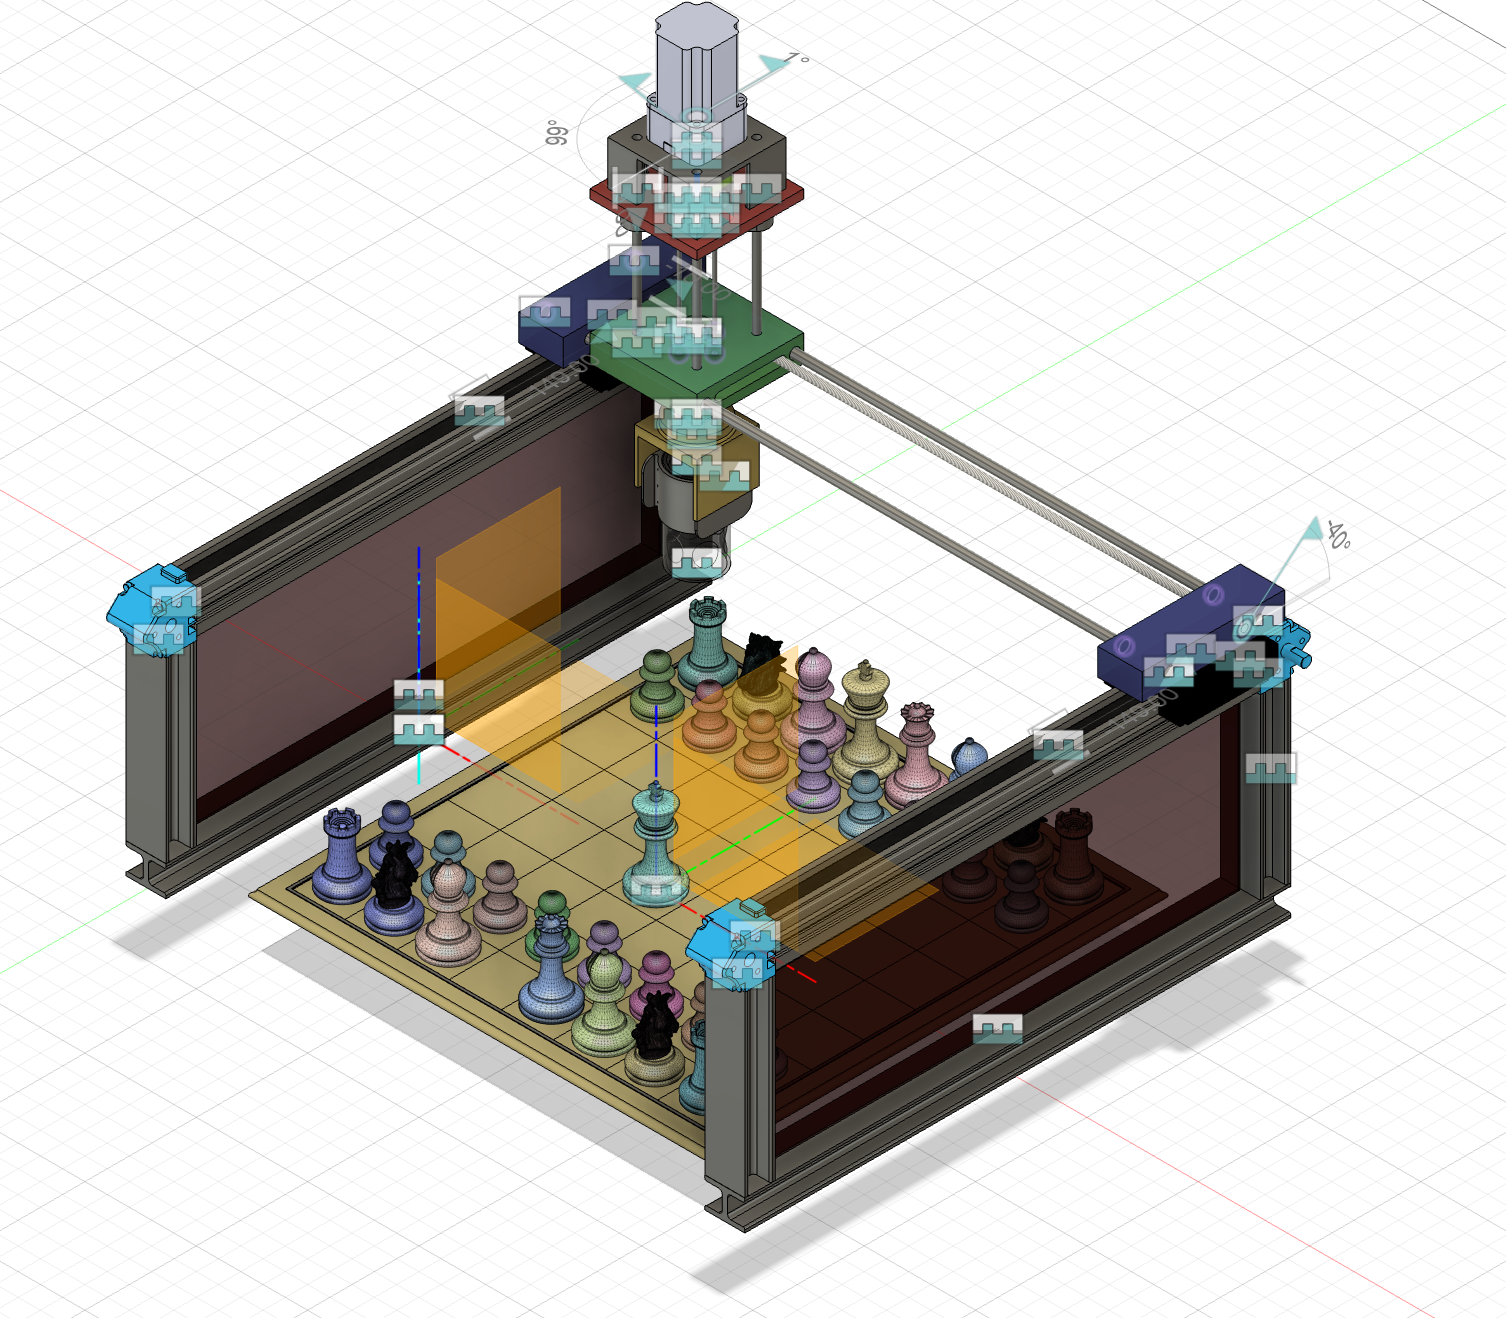
\includegraphics[width=0.8\linewidth]{final design.png}
    \caption{final design of chess playing robot}
    \label{fig:final design}
\end{figure}

\subsection{Frame Stucture}
The frame part of the robot is made of aluminum alloy, and this part is chosen to be produced through casting. Casting offers flexibility in production: it can produce complex-shaped aluminum alloy parts and is suitable for large-scale batch production, making it an excellent choice.

\subsection{End Effector}
As mentioned earlier, the end effector consists of two parts: an external rigid structure and an internal soft actuator. Both of these structural parts are chosen to be completed through injection molding. Injection molding not only has a fast manufacturing speed and low processing cost but is also more conducive to post-processing after production, making it suitable for mass production.

\section{Manufacturing Process Flow}
\subsection{Production of the Frame Structure}
\begin{itemize}
    \item \textbf{Preparation of Casting Process}: This includes selecting the appropriate casting method (such as sand casting, die casting, low-pressure casting, etc.), and preparing the relevant casting equipment and materials.
    \item \textbf{Design and Manufacture of Molds}: Design the mold according to the requirements of the cast part. Molds are usually made of heat-resistant materials that can withstand the high temperatures of aluminum alloy.
    \item \textbf{Melting the Aluminum Alloy}: Heat the aluminum alloy raw material in a furnace to a molten state (660°C to 800°C). This process may involve adding some alloying elements to adjust the material's properties.
    \item \textbf{Pouring}: Remove the molten aluminum alloy from the furnace and pour it into the pre-prepared molds (heated to 200°C to 250°C). This process requires controlling the temperature (680°C to 760°C) and flow rate of the molten aluminum alloy to ensure the quality of the casting.
    \item \textbf{Solidification and Cooling}: The aluminum alloy solidifies in the mold. During this process, the volume of the aluminum alloy will shrink, so this must be considered in the mold design.
    \item \textbf{Demolding and Cleaning}: After the aluminum alloy has completely cooled, remove it from the mold. It may be necessary to remove excess parts such as gates and risers, and to clean and polish the surface.
    \item \textbf{Heat Treatment and Post-Processing}: If necessary, heat treat the casting to improve its mechanical properties. Additionally, surface treatments such as painting or anodizing may be performed to enhance corrosion resistance and appearance.
    \item \textbf{Inspection and Quality Control}: Inspect the casting for dimensions, appearance, and performance to ensure it meets design specifications.
\end{itemize}

\subsection{Production of the End Effector Shell}

\subsubsection{Preparation Stage}
\begin{itemize}
    \item \textbf{Material Selection}: Choose suitable ABS material for the product application, which may include different additives to improve performance.
    \item \textbf{Dry the Raw Material}: ABS pellets typically need to be dried before injection molding to remove moisture, preventing bubbles or other defects during molding.
\end{itemize}

\subsubsection{Injection Molding Stage}
\begin{itemize}
    \item \textbf{Preheat the Machine}: Start the injection molding machine and set the appropriate temperature and pressure parameters. The typical processing temperature range for ABS is between 200°C and 280°C.
    \item \textbf{Injection Molding}: Heat the ABS to a molten state and inject it under high pressure into the preheated mold cavity.
    \item \textbf{Demolding}: After cooling, open the mold and eject or remove the formed part with a mechanical arm.
\end{itemize}

\subsubsection{Post-Processing Stage}
\begin{itemize}
    \item \textbf{Deburring}: Remove residual parts of the runner system and burrs, which can be done manually or mechanically. For batch production, we choose a mechanical removal method - using specialized trimming machines or other mechanical equipment to automatically remove burrs. These devices can trim the burrs of a large number of products quickly and accurately, but require a relatively high initial investment in machinery.
    \item \textbf{Secondary Processing}: Perform drilling, milling, or cutting, etc.
    \item \textbf{Surface Treatment}: Such as painting, screen printing, or gold plating. Due to certain wear resistance requirements, we choose Physical Vapor Deposition (PVD) - applying a thin metal film to improve wear resistance and decoration.
    \item \textbf{Inspection and Testing}: Check dimensional accuracy, appearance, and physical properties to ensure product quality.
\end{itemize}

\subsection{Production of the Soft Actuator}
As is shown in Fig. \ref{fig:demolding_assembly}, four main processes are involved in soft actuator production.
\begin{itemize}
    \item \textbf{Design and Mold Creation}: Design the mold model of the soft robot on a computer, and then carry out 3D printing.
    \item \textbf{Material Preparation:} Measure two components of Eco-flex liquid A and B in a 1:1 ratio. Eco-flex is a silicone rubber commonly used in soft robotics, known for its flexibility and durability. Mix liquids A and B in a container, and stir for one minute to ensure thorough mixing.
    \item \textbf{Pouring Process}: Pour the Eco-flex liquid mixture into the prepared mold (Step 01). It fills the lower cavity of the mold. Then cure the material at a temperature of 70 degrees Celsius for one hour (Step 02) to solidify and form the shape of the mold.
    \item \textbf{Demolding and Assembly}: After the curing process, remove the solidified Eco-flex shape from the mold; this step is called demolding (Step 03). Finally, stick the two cast planes together to form the final component. Eco-flex itself acts as the glue to bond the two parts. After assembly, a cavity is left in the middle of the flat structure.
\end{itemize}

\begin{figure}
    \centering
    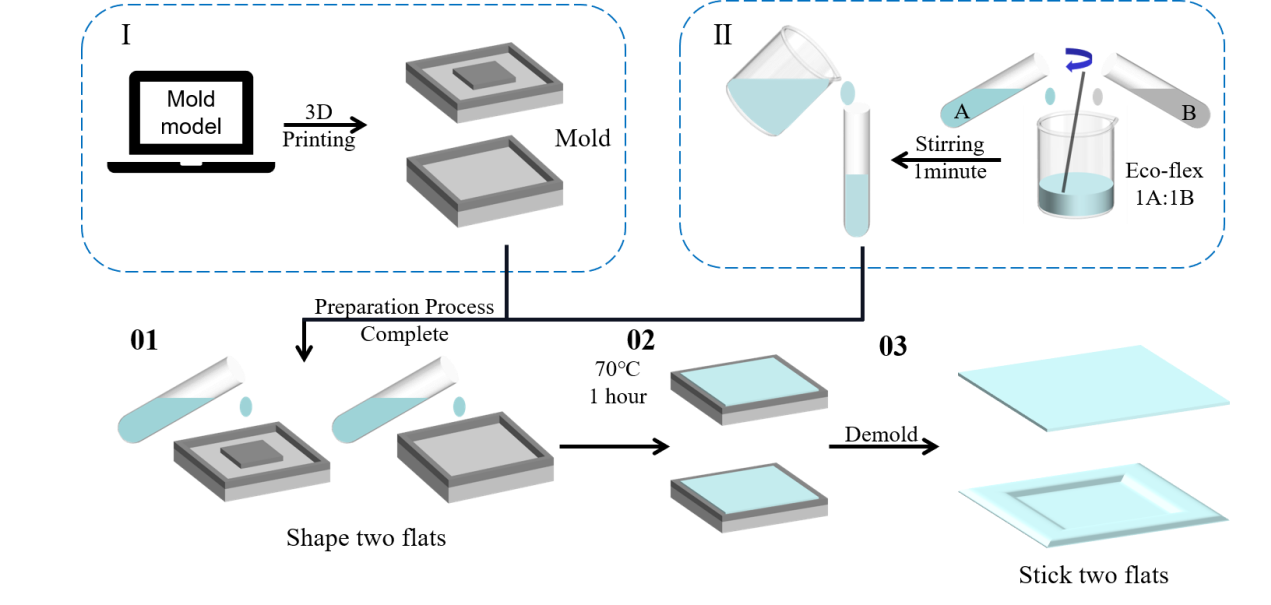
\includegraphics[width=\linewidth]{demolding and assembly.png}
    \caption{process of demolding}
    \label{fig:demolding_assembly}
\end{figure}

By injecting air into the middle cavity, the soft structure expands from flat to the shape of a spherical cap.

\begin{figure}
    \centering
    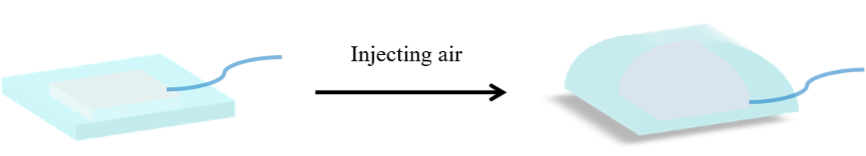
\includegraphics[width=0.8\linewidth]{process of injecting air.png}
    \caption{process of injecting air}
    \label{fig:process of injecting air}
\end{figure}

\section{Assembly}
The focus of this project is on the end effector of this robot, so the emphasis here is on how it is assembled.

The outer shell and the soft structure of the end effector are bonded together using glue. Small holes are drilled in the shell of the end effector, which leads to grooves in the inner wall. Glue can be injected through these holes into the grooves, allowing the internal soft structure to be combined with the outer shell.

\begin{figure}
    \centering
    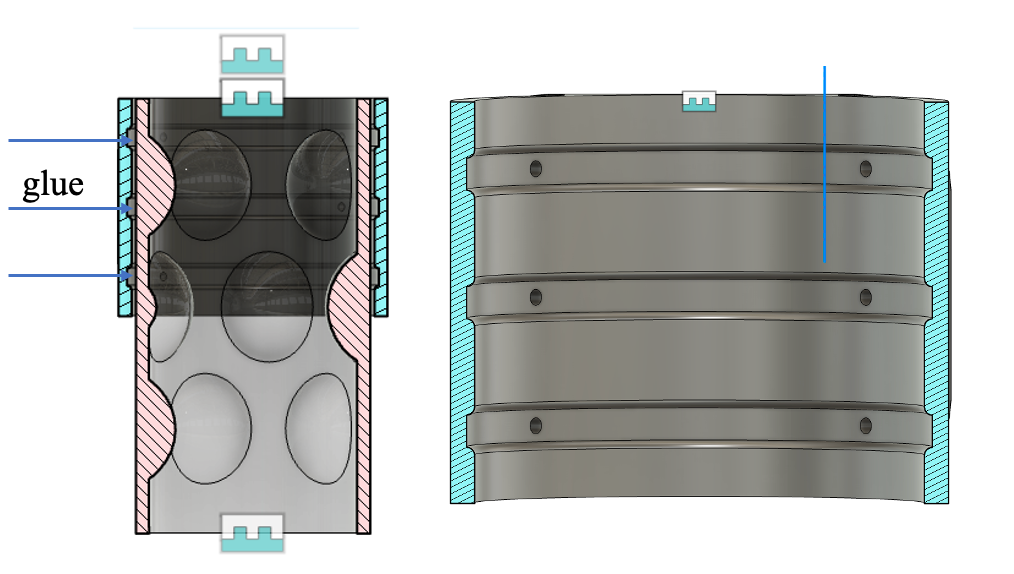
\includegraphics[width=0.8\linewidth]{end effector assembly.png}
    \caption{end effector assembly}
    \label{fig:end effector assembly}
\end{figure}

\bibliographystyle{plain}
\bibliography{ref}

\end{document}

%%%%%%%%%%%%%%%%%%%%%%%%%%%%%%%%%%%%%%%%%%%%%%%%%%%%%%%%%%%%%%%%%%
%%%%%%%%%%%%%%%%%%%%%%%%%%%%%%%%%%%%%%%%%%%%%%%%%%%%%%%%%%%%%%%%%%
